\chapter{Projektin lähtökohdat}
\label{ch:projektin-lähtökohdat}

% TODO: Kirjoita tämä vastaamaan demon analyysia ja muuta otsikko myös vastaamaan sitä. Tästä kappaleesta tuloksena pitäisi tulla tiedot mikä demossa on vikana joita voidaan käytää myöhemmin suunnitelussa.

Tarkoituksena tässä diplomityössä oli toteuttaa ohjelmistokomponentti osaksi isompaa järjestelmää. Isompi järjestelmä liittyi sähköasemien toimintaan ja niiden tarkkailuun. Ohjemistokomponentin tarkoituksena oli tilata viestejä sähköaseman IED-laitteen RCB-instansseilta IEC 61850 -standardin mukaisesti. Standardin mukainen viesti prosessoitiin ja jaettiin järjestelmän muiden komponenttien kanssa. Esimerkiksi viesti voi sisältää mittaustietoa, joka halutaan näyttää loppukäyttäjälle käyttöliittymässä. Käyttöliittymän päivittävä komponentti tarvitsee mittaustiedon IED-laitteelta.

Ennen tämän työn aloittamista yrityksessä oli jo kehitetty ensimmäinen versio ohjelmasta. Ohjelma kykeni tilaamaan viestejä IED-laitteen kaikilta RCB-instansseilta, prosessoimaan viestit ja tallentamaan ne relaatiotietokantaan myöhempää käyttöä varten. Tässä ohjelmistossa oli havaittuja ongelmia ja se ei myöskään tukenut kaikkia IEC 61850 -standardin viesteihin liittyviä ominaisuuksia. Tämän ohjelmiston toimintaperiaate ja siinä olleet ongelmat toimivat pohjana uuden version suunnittelulle ja toteutukselle. Tarkoituksena oli poistaa havaitut ongelmakohdat ja miettiä olisiko jokin muu arkkitehtuuri parempi kyseiseen toteutukseen. Ensimmäistä toteutusta ohjelmasta voisi nimittää ensimmäiseksi protoversioksi tai demovaiheeksi (engl. proof of concept), jonka pohjalta tultiin tekemään toimiva lopullinen versio. Tekstissä eteenpäin sanoilla demo ja demoversio viitataan tähän ohjelmistoon.

Tässä osiossa pohjustetaan työn alkua lukijalle ja mistä lähdettiin liikkeelle. Lisäksi kuvataan mitä ongelmia demovaiheen toteutuksessa ja oli ja analysoida niitä. Demovaiheen ohjelmasta käsitellään sen arkkitehtuuria, mitkä olivat sen komponentit ja niiden toiminnallisuus. Tässä käsitellyt ongelmat toimivat pohjana uuden version suunnittelulle ja auttavat tekemään siihen liittyviä ratkaisuja.


\section{Demon arkkitehtuuri}
\label{ch:demoversio-ja-sen-toiminta}
Demoversio oli ohjelmoitu Ruby-ohjelmointikielellä. Ohjelman arkkitehtuuri oli yksinkertainen. Kuvassa \ref{fig:demo-architecture} on esitetty demoversion arkkitehtuuri korkealla tasolla ja kuinka viesti IED-laitteelta kulkee tietokantaa. Yksi ajettu demoversion prosessi pystyi tilaamaan yhden IED-laitteen kaikki RCB-luok\-ki\-en instanssit. Instanssien tiedot luettiin relaatiotietokannasta. Ohjelmisto prosessoi viestit ja tallensi ne relaatiotietokantaan myöhempää käyttöä varten. Ruby-ohjelmistossa tärkeässä osassa oli \emph{libIEC61850}-kirjasto \cite{libIEC61850-homepage}. libIEC61850-kirjasto on avoimen lähdekoodin C-kielellä toteutettu kirjasto, joka abstrahoi IEC 61850 -standardin matalan tason määrittämiä palvelukutsuja ja datarakenteita helppokäyttöiseksi rajapinnaksi. Kirjasto tarjosi toiminnallisuuden IED-laitteella olevan palvelinohjelmiston, sekä IED-laitetta käyttävän asiakasohjelmiston toteuttamiseen. IED-laitteen palvelimelle kirjasto tarjosi funktioita ja rakenteita IEC 61850 määrittämien luokkien ja hierarkian rakentamiseen ja käsittelyyn. IED-laitteen asiakasohjelmalle kirjasto tarjosi funktioita ja rakenteita standardin määrittämiin palveluihin, kuten arvojen lukuun ja asettamiseen, datajoukkojen käyttöön ja viestien tilaamiseen. Tätä samaa kirjastoa käytettiin myös tässä työssä toteutetussa ohjelmistokomponentissa. Demossa ja lopullisessa ohjelmistokomponentissa käytettiin vain kirjaston tarjoamia IED-laitteen asiakasohjelmiston ominaisuuksia

\begin{figure}[ht!]
	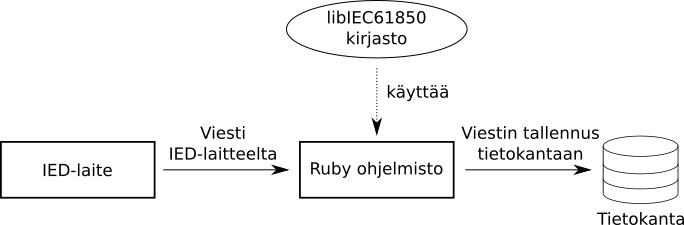
\includegraphics[width=1\textwidth]{pictures/demo-architecture.png}
	\caption{Rubylla toteutetun demoversion arkkitehtuuri ja tiedonsiirto.}
	\label{fig:demo-architecture}
\end{figure}

LibIEC61850-kirjasto on rakennettu käyttämään MMS-protokollaa tiedonsiirrossa IED-laitteen ja sen asiakasohjelman välillä, kuten IEC 61850 -standardin osassa 8-1 määritetään. Kuvassa \ref{fig:libiec61850-layer-architecture} on esitetty kirjaston kerrosarkkitehtuuri asiakasohjelmalle. Kirjastoon on toteutettu \emph{laiteabstraktiokerros} (engl. \emph{Hardware Abstraction Layer}, lyhennetään \emph{HAL}). HAL:in avulla kirjasto voi toimia monella eri laitealustalla, ja käyttäjä voi tarvittaessa lisätä oman HAL-implementaation. Demoversiota suoritettiin Linux-käyttöjärjestelmällä, joten kirjastosta käytettiin olemassa olevaa Linux HAL -toteutusta. Kuvassa \ref{fig:libiec61850-layer-architecture} on punaisella merkitty laatikot, jotka kirjaston käyttäjä voi tarjota itse, keltaisella kirjaston uudelleenkäytettävät MMS-protokollan osuudet ja sinisellä IEC 61850 -standardin toteuttavat osuudet. Kuvaan on merkitty vihreällä demoon toteutetut osuudet, eli Ruby-kielelle liitos C-kieleen ja tämän päälle Rubylla tehty ohjelmisto.

\begin{figure}[ht!]
	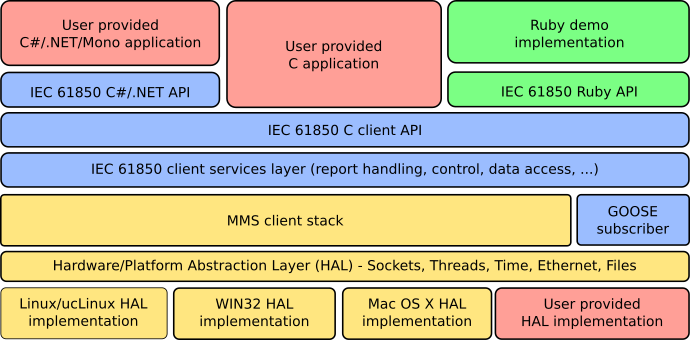
\includegraphics[width=1\textwidth]{pictures/libiec61850-layer-architecture.png}
	\caption{libIEC61850-kirjaston kerrosarkkitehtuurin komponentit, vihreällä Ruby toteutukseen lisätyt osat (pohjautuu kuvaan \mbox{\cite{libIEC61850-api-overview}}).}
	\label{fig:libiec61850-layer-architecture}
\end{figure}

Ruby-koodista C-kielen funktioiden kutsuminen ei ole suoraan mahdollista, vaan kielten väliin täytyy toteuttaa liitos. Demoversiossa liitos oli tehty käyttäen Rubylle saatavaa \emph{ruby-ffi} -kirjastoa \cite{ruby-ffi-repo} (engl. \emph{Foreign Function Interface}, lyhennetään \emph{FFI}). Liitoksen avulla Ruby voi kutsua C-kielen funktioita ja käyttää sen struktuureita ja muuttujia. Demossa kirjasto huolehti matalan tason IEC 61850 asiat, ja Ruby-koodi keskittyi liitoksen avulla korkean tason viestin jäsentämiseen ja tallennukseen tietokantaan.


\section{Demon toiminta ja sen ongelmat}
\label{ch:ongelmakohdat-ja-analysointi}
Demo oli toteutettu käyttäen \emph{Ruby on Rails} -kehystä, lyhennetään \emph{RoR}. RoR on tarkoitettu web-sovellusten toteuttamiseen Ruby-kielellä. Se tarjoaa \emph{Active Record} -nimisen \emph{ORM}-kerroksen (engl. \emph{Object-Relational Mapping}) tietokannan käsittelyn helpottamiseen. ORM-kerros abstrahoi relaatiotietokannan käyttämisen oliopohjaiseksi ja kyselyitä tietokantaan voi tehdä suoraan Ruby-kielellä. Demo käytti RoR:in ORM-kerrosta tietokannan käyttämiseen. Demossa päädyttiin käyttämään RoR-kehystä, koska muu järjestelmä oli toteutettu tällä kehyksellä. Ennen suorittamista ohjelmaan täytyi ladata RoR:in ympäristö muistiin, jonka seurauksena yksinkertaisen ohjelman piti varata iso määrä muistia.

Ohjelman toiminta on esitetty sekvenssikaavioissa \ref{fig:sequence-diagram-report-subscription} ja \ref{fig:sequence-diagram-report-subscription-processing}. Sekvenssikaavio \ref{fig:sequence-diagram-report-subscription} jatkuu kuvassa \ref{fig:sequence-diagram-report-subscription-processing}. Kuvissa ohjelman kaksi eri silmukkaa on esitetty loop-laatikoilla. Sekvenssikaaviossa osallisena ovat tietokanta, Ruby-ohjelma, libIEC61850-kirjasto, libIEC61850-kirjaston natiivisäie ja IED-laitteen palvelinohjelma. Rubyn ja libIEC61850-kirjaston liitos oli tehty ruby-ffi -kirjastolla ja kirjaston natiivisäie oli vastuussa yhteyden ylläpidosta ja datan siirtämisestä. Sekvenssikaavioon on merkitty paksulla suorituksessa olevat palkit, esimerkiksi IED-laitteen palvelinohjelmisto on koko ajan suorituksessa. Tulevassa tekstissä viitataan molempien kuvien kohtiin numeroilla.

\begin{figure}[ht!]
	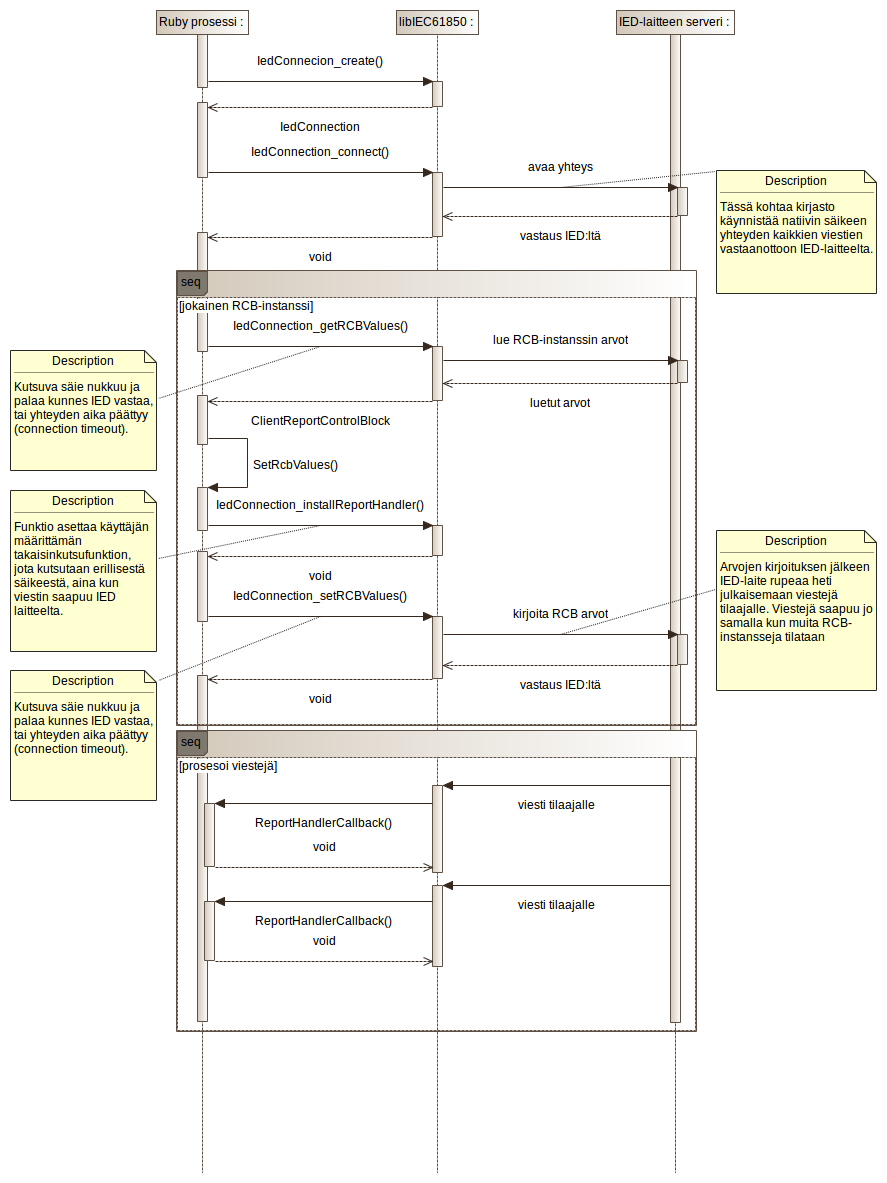
\includegraphics[width=1\textwidth]{pictures/sequence-diagram-report-subscription.png}
	\caption{Sekvenssikaavio kuinka Ruby-ohjelma avaa yhteydet ja tilaa kaikki IED-laitteen RCB-instanssit (jatkuu kuvassa \ref{fig:sequence-diagram-report-subscription-processing}).}
	\label{fig:sequence-diagram-report-subscription}
\end{figure}

\begin{figure}[ht!]
	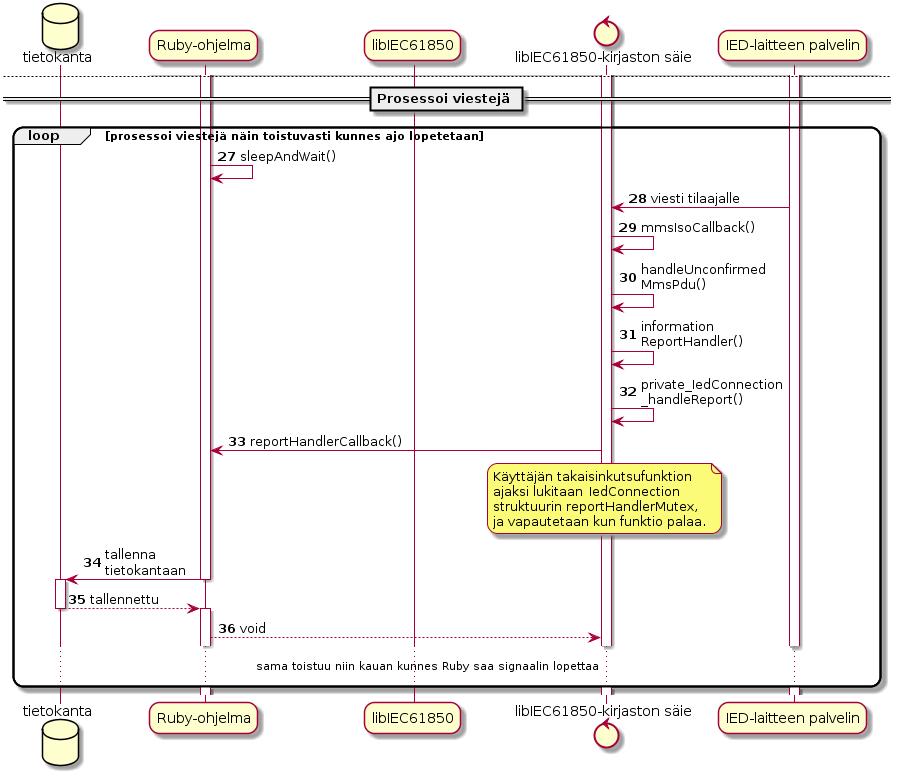
\includegraphics[width=1\textwidth]{pictures/sequence-diagram-report-subscription_001.png}
	\caption{Sekvenssikaavio kuinka Ruby-ohjelma prosessoi ja tallentaa viestejä libIEC61850-kirjastoa käyttäen (jatkuu kuvasta \ref{fig:sequence-diagram-report-subscription}).}
	\label{fig:sequence-diagram-report-subscription-processing}
\end{figure}

IED-laiteella viestejä mahdollisesti generoidaan ja lähetetään samaan aikaan. Seurauksena niitä voi saapua libIEC61850-kirjastolle ennen kuin edellinen viesti on käsitelty. Tätä varten kirjasto toteuttaa sisäisen puskurin viestien vastaanottamiseen. Puskurista prosessoidaan seuraava viesti kun edellinen on prosessoitu. Toisin sanoen kirjasto ottaa viestejä vastaan sitä mukaan kun ne saapuu ja ottaa niitä puskurista yksi kerrallaan saapumisjärjestyksessä. Kirjasto varaa yhden puskurin avattua yhteyttä kohti. Jos ohjelma avaa vain yhden yhteyden, kirjaston käyttäjän ei tarvitse huolehtia rinnakkaisuudesta. \cite{libIEC61850-repo}

Ensimmäisenä ohjelma luki tietokannasta IED-laitteen, sekä sen kaikki RCB-instanssien tiedot. Tämän avulla ohjelma tiesi mikä IED-laitteen IP-osoite on ja mitkä olivat RCB-instanssien viitteet (kohdat 1--2). Ohjelmaan pystyi syöttämään eri tietoja ainoastaan tietokannan kautta ennen suoritusta. Tämän jälkeen ohjelma pystyi muodostamaan yhteyden IED-laitteelle tekemällä instanssin \texttt{IedCon\-nec\-ti\-on} struktuurista funktiolla \texttt{Ied\-Con\-nec\-ti\-on\_crea\-te\-()} (kohdat 3--4). Tämän jälkeen struktuuri annetaan \texttt{Ied\-Con\-nec\-ti\-on\-\_\-con\-nect\-()} funktiolle, joka avaa yhteyden IED-laitteelle ja palaa vasta kun vastaus saapuu (kohdat 5--11). Tässä vaiheessa libIEC61850-kirjasto käynnistää erillisen natiivisäikeen yhteyden viestien vastaanottoon. Tätä säiettä kirjasto käyttää tulevien viestien vastaanottoon ja lähettämiseen. Yhteyden avauksen jälkeen jokainen RCB-instanssi tilataan lukemalla ensin sen arvot IED-laitteelta funktiolla \texttt{Ied\-Con\-nec\-ti\-on\-\_\-get\-RCB\-Va\-lu\-es\-()} (kohta 12). Funktiokutsu nukkuu ja palaa vasta kunnes erillinen säie ilmoittaa, että vastaus on saapunut tai yhteyden aika ylittyy. Kirjaston funktio  \texttt{send\-Re\-qu\-est\-And\-Wait\-For\-Res\-pon\-se\-()} nukkuu ja odottaa vastausta (kohdat 13--16). RCB-arvot luettuaan, kirjasto palauttaa struktuurin \texttt{Cli\-ent\-Re\-port\-Cont\-rol\-Block}, joka sisältää luetut tiedot RCB-instanssista (kohta 17). Samaa struktuuria käytetään arvojen muuttamiseen ja niiden takaisin kirjoittamiseen IED-laitteelle. Ennen muunneltujen RCB-arvojen takaisin kirjoittamista ja viestien tilaamista, täytyy kirjastolle asettaa takaisinkutsufunktio, jota kirjasto kutsuu aina kun tilattu viesti saapuu IED-laitteelta. Takaisinkutsufunktioksi asetetaan funktiolla \texttt{Ied\-Con\-nec\-ti\-on\-\_\-ins\-tall\-Re\-port\-Hand\-ler\-()} (kohdat 19--20). Asetuksen ajaksi kirjasto lukitsee \texttt{re\-port\-Hand\-ler\-Mu\-tex}:in. Tätä samaa lukitusta käytetään kun viesti takaisinkutsufunktiota kutsutaan viestin saapuessa (kohdat 33--36). Tilanteessa jossa takaisinkutsufunktiota asetetaan samalla kun viesti on saapunut, joutuu toinen osapuoli odottamaan lukituksen vapautumista. Tämä lukitus on tärkeä huomio myöhemmin kun käydään läpi ohjelman huonoa suorituskykyä. Tämän jälkeen arvot kirjoitetaan takaisin IED-laitteelle funktiolla \texttt{Ied\-Con\-nec\-ti\-on\-\_\-set\-RCB\-Va\-lu\-es\-()} (kohdat 21--26). Tämä funktio palaa vasta kun IED vastaa tai yhteyden aika ylittyy. Heti arvojen kirjoitusten jälkeen IED aloittaa lähettämään viestejä tilaajalle. Eli samalla kun muita RCB-instansseja tilataan, tilatut RCB-instanssit lähettävät jo viestejä ja aiheuttavat takaisinkutsufunktion suorittamisen. Kun kaikki RCB-instanssit on tilattu, ohjelma jää viimeiseen silmukkaan odottamaan ja prosessoimaan viestejä (kohdat 27--36). Kun viesti saapuu, säie kutsuu ensin sisäisesti \texttt{mms\-I\-so\-Call\-back\-()} funktiota, joka kutsuu muita kirjaston sisäisiä funktioita ja lopuksi asetettua takaisinkutsufunktiota (kohdat 28--33). Takaisinkutsufunktio on liitetty Ruby funktioon ja funktio tallentaa raportin tiedot tietokantaan (kohdat 33--36). Ruby-funktion suorituksen ajaksi kirjasto lukitsee \texttt{re\-port\-Hand\-ler\-Mu\-tex}:in, ja vapautetaan kunnes Ruby-funktion suoritus palaa. Tätä jatkuu niin kauan kunnes ohjelmalle lähetetään jokin signaali joka lopettaa sen suorituksen. \mbox{\cite{Kozlovski2017, Storimer2013, libIEC61850-repo}}

Demossa isoimpana ongelmana oli sen huono suorituskyky ja toiminnan epävarmuus RCB-instanssien määrän ollessa enemmän kuin muutama. RCB-instanssien määrän ollessa liian suuri ohjelma saattoi epäonnistua osan tilaamisessa, koska yhteys aikakatkaistiin arvojen kirjoituksessa tai luvussa. Lisäksi ongelmaksi muodostui usean RCB instanssin tilaamisen kulunut aika. Yhteensä aikaa saattoi kulua 30 sekuntia kaikkien instanssien tilaamiseen.

Huonoon suorituskykyyn oli syynä muutama asia. Yksi niistä oli Ruby-kielen huonompi suorituskyky verrattuna natiivisti käännettyyn C-kieleen. Ruby on tulkattava kieli kuten esimerkiksi Python, joka tulkataan rivi kerrallaan ja suoritetaan. Lähdekoodia ei käännetä kokonaan ensin konekäskyiksi erillisellä kääntäjällä, kuten C-kielessä. Valmiiksi käännetty lähdekoodi tarvitsee vain ajaa, kun taas tulkattavassa kielessä rivi täytyy ensin tulkata ja sitten ajaa. Rubyssa käytettiin sen oletustulkkia \emph{MRI/YARV} (engl. \emph{Matz's Ruby Interpreter}, lyhennetään \emph{MRI} tai \emph{Yet another Ruby VM}, lyhennetään \emph{YARV}). Ruby versiosta 1.9 eteenpäin käyttää YARV-tulkkia. Toinen syy oli Ruby-kielen oletustulkissa oleva \emph{globaali tulkkilukitus} (engl. \emph{Global Interpreter Lock}, lyhennetään \emph{GIL}, tai \emph{Global Virtual Machine Lock}, lyhennetään \emph{GVL}). GIL pakottaa Ruby-ohjelman ajoon vain yhdellä ytimellä ja vain yksi säie vuorossa kerrallaan ja on täysin riippumaton käyttöjärjestelmän vuorottajasta \mbox{\cite[s.~131--133]{Odaira2014}}. Kuvassa \ref{fig:ruby-gil} on esitetty kuinka Ruby-tulkki vuorottaa kahta ajossa olevaa säiettä. Kuvassa demon Ruby-koodi kutsuu \texttt{Ied\-Con\-nec\-ti\-on\-\_\-set\-RCB\-Va\-lu\-es\-()} funktiota, ajo jää kesken ja tapahtuu vaihto, koska viesti saapui. Takaisinkutsufunktio suoritetaan ja suoritus palaa takaisin aikaisempaan funktion suoritukseen. Tässä vaiheessa jos vaihto on huonolla hetkellä ja kesti liian kauan, tulee yhteyden aikakatkaisu ja RCB-instanssi jää tilaamatta. Huonoon suorituskykyyn mahdollisesti vaikutti myös lukitus \texttt{re\-port\-Hand\-ler\-Mu\-tex}, jota kirjastossa käytetään kun takaisinkutsufunktio asetetaan tai sitä suoritetaan. Lukitus aiheuttaa säikeen nukkumisen niin kauan kunnes lukitus vapautuu. Tässä tapauksessa, jos viestin prosessointi kestää liian kauan (kuvassa \ref{fig:sequence-diagram-report-subscription-processing} kohdat 33--36) ja samalla tilataan muita RCB-instansseja (kuvassa \ref{fig:sequence-diagram-report-subscription} kohdat 12--26). Säie joutuu odottamaan lukituksen vapautusta takaisinkutsufunktion asetettamisen ajan (kohdat 19--20). Ratkaisuna tähän olisi pitää takaisinkutsufunktio mahdollisimman lyhyenä suoritusajan suhteen.

\begin{figure}[ht!]
	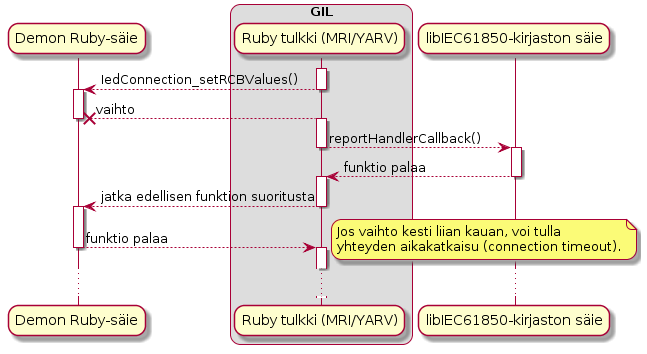
\includegraphics[width=1\textwidth]{pictures/ruby-gil.png}
	\caption{Ruby-tulkin globaalin lukituksen toiminta, joka vuorottaa ajossa olevia säikeitä riippumatta käyttöjärjestelmän vuorottajasta.}
	\label{fig:ruby-gil}
\end{figure}

Tämän lisäksi demototeutuksessa oli muistivuoto. Muistivuoto on tilanne, missä ohjelma varaa kokoajan lisää muistia eikä vapauta sitä takaisin käyttöjärjestelmälle uudelleen käyttöön. Muistivuoto johtui todennäköisesti jostakin ohjelmointivirheestä ruby-ffi -kirjaston liitoksen kanssa. Kun liitos Rubysta tehdään C-kieleen, täytyy ohjelmoijan miettiä roskien keruuta tarkasti. Tätä ei normaalisti tarvitse miettiä Rubyssä, koska tulkki implementoi automaattisen roskien keruun. Muistivuoto havaittiin kun ohjelma jätettiin suoritukseen pitemmäksi aikaa ja ohjelma oli varannut melkein kaiken käyttöjärjestelmän muistista itselleen. Lisäksi jos ohjelmaa ajaa ja tarkkailee Linuxin \emph{htop}-ohjelmalla, voi \emph{MEM\%}-sarakkeesta huomata prosentuaalisen osuuden kasvavan koko käyttöjärjestelmän muistista.

Näiden lisäksi tiedon jako järjestelmän muiden komponenttien kanssa oli huono. Ohjelma prosessoi viestit relaatietokantaan. Muiden komponenttien täytyi kysellä tietoa tietokannasta tasaisin väliajoin, ilman tietoa milloin uusi tieto on saatavissa. Komponenttien määrästä riippuen tietokanta on turhan rasituksen alaisena jatkuvasti. Tulevaisuutta ajatellen lopullinen tiedon tallennuspaikka ei ole muiden tietoa tarvitsevien ohjelmien kannalta järkevä. Tarvittaisiin keino, jolla komponentit voisivat saada tiedon uudesta viestistä erikseen, ilman että sitä täytyisi kysellä väliajoin.